\documentclass[a4paper]{jarticle}
\usepackage{sice-si}
\usepackage{amsmath} 
\usepackage[dvipdfmx]{graphicx}


\begin{document}
%
% タイトルと著者名
\title{音声中に出現する特定キーワードの自動ゲイン調整を行う装置の開発} % 和文タイトル
\name{○佐々部 岳人,天野 俊一(流通経済大学)} % 著者名
\etitle{Development of a device that automatically adjusts the gain of specific keywords that appear in speech.} % 英文タイトル
\ename{○Gakuto Sasabe, and Shunichi Amano (Ryutsu Keizai University)}	%著者名(英)
%
% アブストラクト
\abst{
When we obtain information visually, it is possible to filter only the information we want to obtain, for example, by using a recommendation function for online shopping. On the other hand, in the auditory sense, technologies that uniformly cut noise in specific frequency bands in the outside world, such as noise cancellation, have been put to practical use, but there are still few technologies that cut specific information such as keywords that appear in speech. If such technology is put to practical use, it is expected to contribute to the improvement of productivity and creativity in work involving listening. In this study, we will develop a system that automatically adjusts the gain of speech corresponding to specific keywords. We will also examine the effect of this system on the user's task performance.
}
% タイトルの出力
\maketitle
%
% 本文
\section{緒言}
本稿では SICE SI 部門講演会 SI の予稿原稿を作成するための説明を行います.
SIでは予稿原稿としてPDFファイル形式のファイルを電子投稿していただくことを原則とさせていただいております.
ただし,電子化やネットワーク接続が困難な場合には個別に対応させていただきますので,プログラム委員会までご相談ください(Webサイトからお問い合わせできます).
%
\section{自動ゲイン調整装置}
\begin{figure}[htbp]
    \begin{center}
    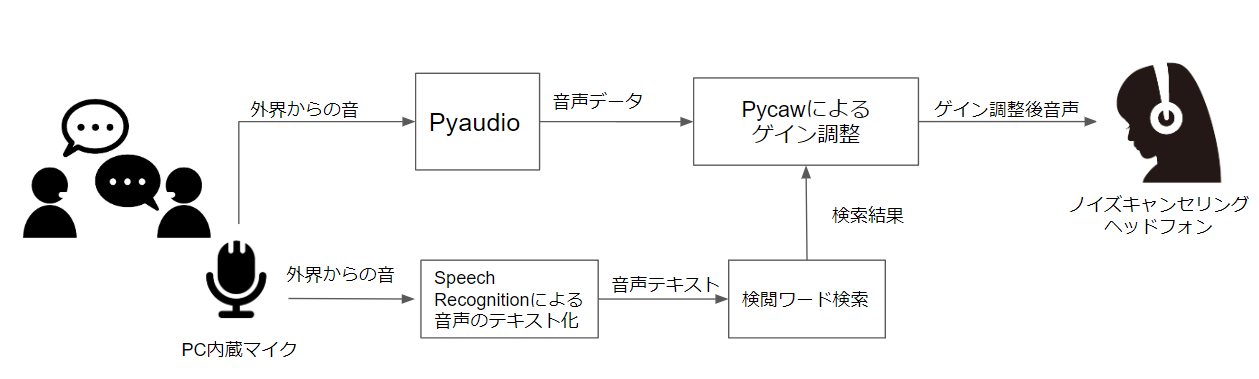
\includegraphics[width=80mm]{system.PNG}
    \caption{The device and the configuration.}
    \label{fig:system}
    \end{center}
    \end{figure}

本研究で提案する装置の構成をFig.\ref{fig:system}に示す.
本装置はワイヤレスヘッドフォン(ag製 WHP01K),PC(DELL製 ALIENWARE 13(R3)),マイク(ALIENWARE 13(R3)内蔵マイク)によって構成される.
PCには,Pythonにより記述されたシステムが搭載されており,これによってマイクから入力される音に対して自動でゲイン調整を行う.
ワイヤレスヘッドフォンはノイズキャンセリング機能を有し,装置使用時はノイズキャンセリング機能を常にONの状態としている.
すなわちユーザーは外界からの音をマイクへの入力によってのみ得ることとなる.マイクへの入力として,基本的に人間による発話を想定している.
装置のマイクに入力された音声が,ゲイン調整されてユーザーに届くまでのシステム内の流れについて以下に述べる.
まず,マイクに入力された音声は,Google社のSpeech recognitionによってテキスト化される.(Fig.\ref{fig:system}の下部)
次に,生成されたテキストは検閲ワード検索クラスに送られ,あらかじめ設定された検閲ワードがテキスト中に含まれていないかどうか検索が行われる.
もしテキスト中に検閲ワードが含まれていた場合は,含まれていた検閲ワードと,検閲ワードを見つけたという情報がゲイン調整クラスに送られる.
一方で,マイクに入力された音声はPythonライブラリ"Pyaudio"によってチャンクごとの音声データに分けられ,ゲイン調整クラスに送られる.(Fig.\ref{fig:system}の上部)
ゲイン調整クラスでは,同じくPythonライブラリ"Pycaw"によって音声のゲイン調整が行われる.
このゲイン調整の度合いは発見した検閲ワードの種類に応じてあらかじめ設定することができる.(例えば,”こんにちは”というワードを検閲ワードとし,ゲインを0とするトリガーとすることが事前に設定できる)
最後にゲイン調整済の音声がワイヤレスヘッドフォンに送られ,ユーザーは音声を聞くことができる.
\section{自動ゲイン調整装置の検証実験}
\subsection{装置による音のカットの確認}
\subsubsection{実験概要}
\subsubsection{実験結果}
\subsection{自動ゲイン調整装置がユーザーのタスク遂行に与える影響}
\subsubsection{実験概要}
システムがユーザーのタスク遂行に与える影響を調べるため,4人の男女(男性:3人,女性:1人)に対してAlternative Uses Test(参考文献)を行った.
Alternative Uses Test(以下AUT)とは,被験者に日用品の新たな使い方のアイデアを思いつく限り解答させるタスクである.
例えばお題が「鉛筆」であれば通常用途として「メモを取る」等が考えられるが代替用途は,「黒板を示すのに使う」「箸の代わりとして使う」などである.
(創造性の評価指標を乗せる?)
今回は,人が発話している環境下で装置がユーザーのタスク遂行に与える影響を測るため,AUTの最中に実験者からアイデア出しに関するアドバイスを行った.
\subsubsection{実験環境}
実験は対面で行い,実験者の対面に被験者が座った.実験の様子を図〇に示す.
実験中,被験者の斜め前に設置されたビデオカメラ(DJI製 Osmo Pocket)により,各人の頭部,胸部運動の様子を映像として記録した.
記録したデータは各人の活動量の産出と評価のために使用された.

\subsubsection{実験の流れ}
実験の流れを以下に示す
\begin{enumerate}
    \item 被験者が装置を装着する
    \item 実験者が被験者にAUTの実施方法を説明する
    \item 実験者が被験者にお題を伝え,実験者からの「はじめてください」の言葉でAUTを始める
    \item 随時,実験者から被験者に対してアイデア出しに関するアドバイスを伝える
    \item AUTを始めてから3分後,実験者からの「おわってください」の言葉でAUTを終了する
    \item (2)から(4)をもう一度繰り返す
\end{enumerate}
被験者は,AUTのお題として1回目の試行では「ボールペン」,2回目の試行では「靴下」についてアイデア出しを行うように指示された.
実験中に出たアイデアはA4用紙に印刷されたフォームに逐次記入させた.
また,AUT実施中の実験者からのアドバイスはお題に関するもの(お題が靴下であれば「素材が布であることを考えると面白いアイデアが思いつくかもしれません.」等)と,
お題によらないもの(「誰が使うかを考えてみるといいアイデアが思いつくかもしれません」等)を組み合わせて,AUT開始から30秒毎に一言ずつ計5回行った.
実験後,被験者には簡単な心理アンケートに答えてもらった.
アンケート結果は被験者のアイデア出しへの自己評価や,実験者に対する印象などを調査するために使用された.

\subsubsection{実験条件}
実験を行うにあたりシステム強使用条件とシステム弱使用条件の2つの条件を設け,それぞれの条件につき2人ずつ実験に参加してもらった.
なお,被験者は自分がどちらの条件の被験者になったかは知らされなかった.
システム強使用条件では,「はじめてください」というキーワードをゲインを0%(無音状態)にするトリガーとし,
「終わってください」というキーワードをゲインを100%(制限なし状態)とするトリガーにした.
すなわち,システム強使用条件では,具体的な実験に対する説明以外の,AUTをおこなっている部分ではマイクに入力された音が全てカットされた.
また,システム弱使用条件では,ゲイン調整を行うトリガーを設けず,実験の全ての段階でマイクに入力された音声はそのまま被験者に届いた.

\subsubsection{実験結果}
\section{ディスカッション}
%
%
%参考文献
\begin{thebibliography}{99}
\bibitem{SI}
	計測太郎,制御花子:
	``SICE SI予稿原稿の書き方(サンプル)'',  
   {\it 計測自動制御学会SI部門講演会SICE-SI予稿集}, 
    pp.0000--0000 (20??)
\end{thebibliography}
%
%
%
\end{document}

